First choose which repository to analyze, it is rather obvious initial step, however.
I choose to test it on my old repository
\href{https://github.com/kolosovpetro/IoC-Container}{\texttt{github.com/kolosovpetro/IoC-Container}}.

\subsection{Login to the SonarCloud}\label{subsec:login-to-the-sonarqube}
Next we login to the \href{https://sonarcloud.io/}{\texttt{sonarcloud.io}} using your GitHub account
\begin{figure}[H]
    \centering
    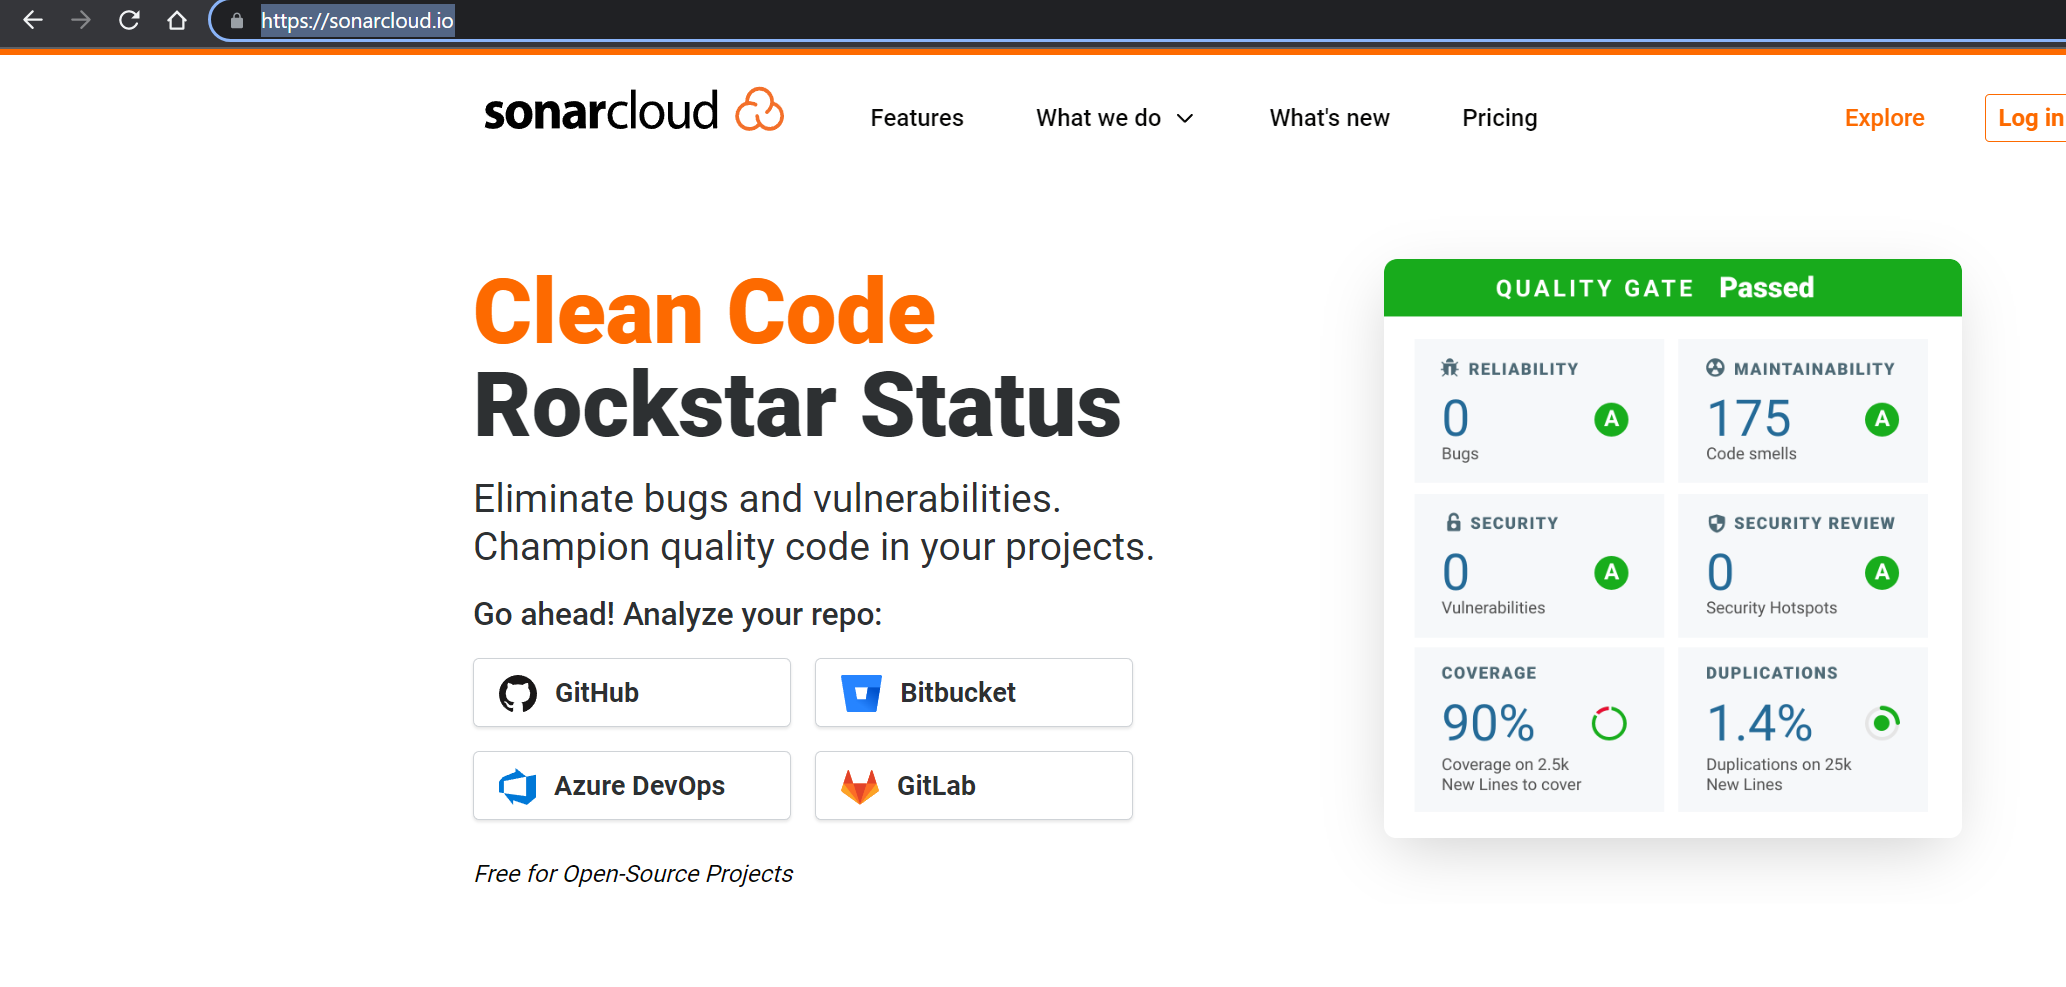
\includegraphics[width=1\textwidth]{img/01_sonarcloud_login_page}
    ~\caption{SonarCloud login page. Use login via GutHub.}\label{fig:figure}
\end{figure}

\subsection{Create an organization at SonarCloud}\label{subsec:create-an-organization-at-sonarcloud}
Now we create an organization we use to analyze your project, I created it as
\begin{center}
    \texttt{petro-kolosov-own-repos}
\end{center}
\begin{figure}[H]
    \centering
    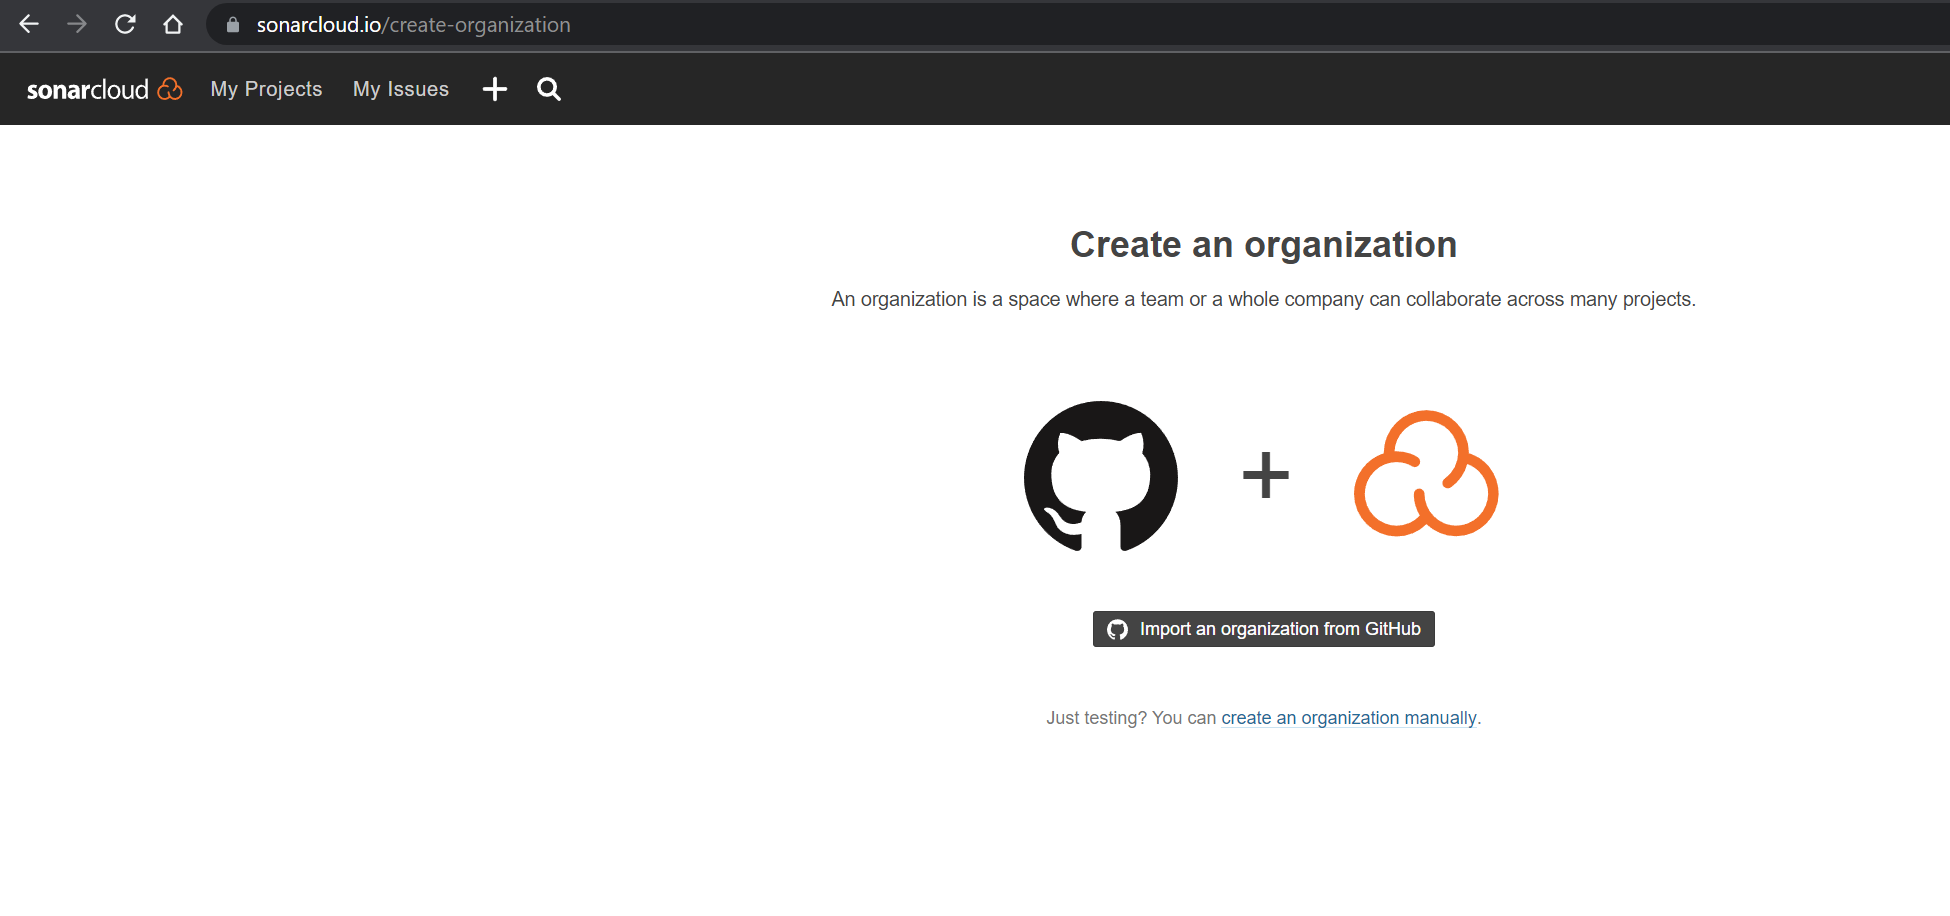
\includegraphics[width=1\textwidth]{img/02_create_organization}
    ~\caption{Create organization form, use \texttt{create an organization manually} at the bottom.}\label{fig:figure2}
\end{figure}
Then enter the key of the organization
\begin{figure}[H]
    \centering
    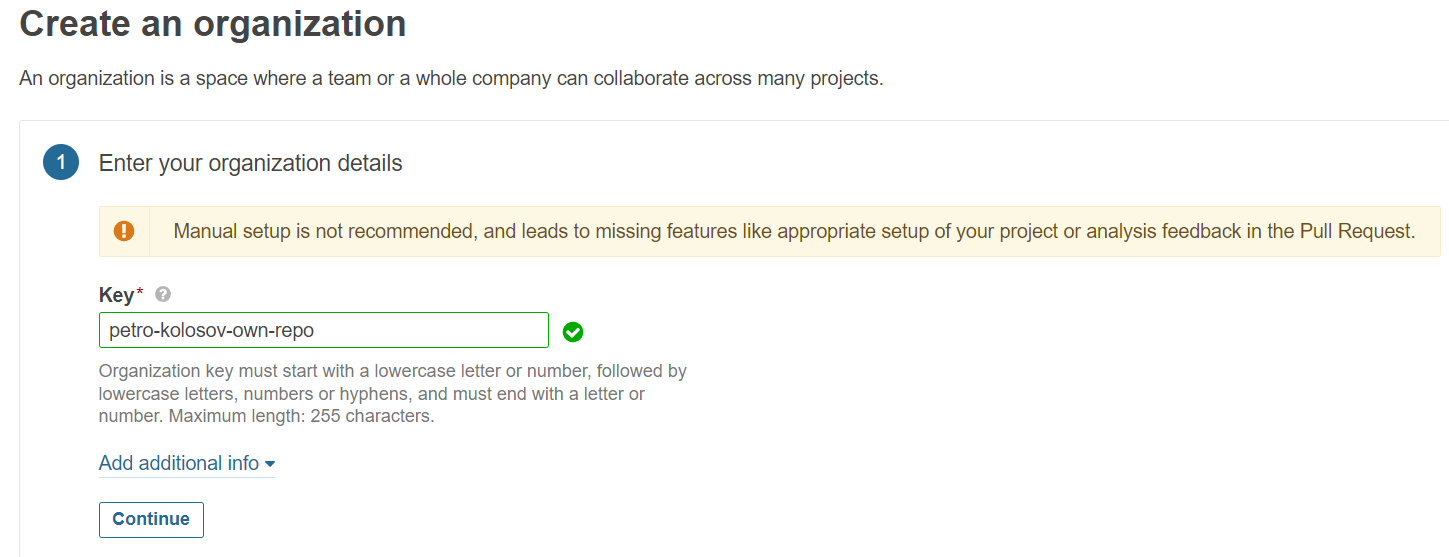
\includegraphics[width=1\textwidth]{img/03_create_organization_key}
    ~\caption{Enter the key of the organization.}\label{fig:figure3}
\end{figure}
Next, choose a plan for your organization, I use free one
\begin{figure}[H]
    \centering
    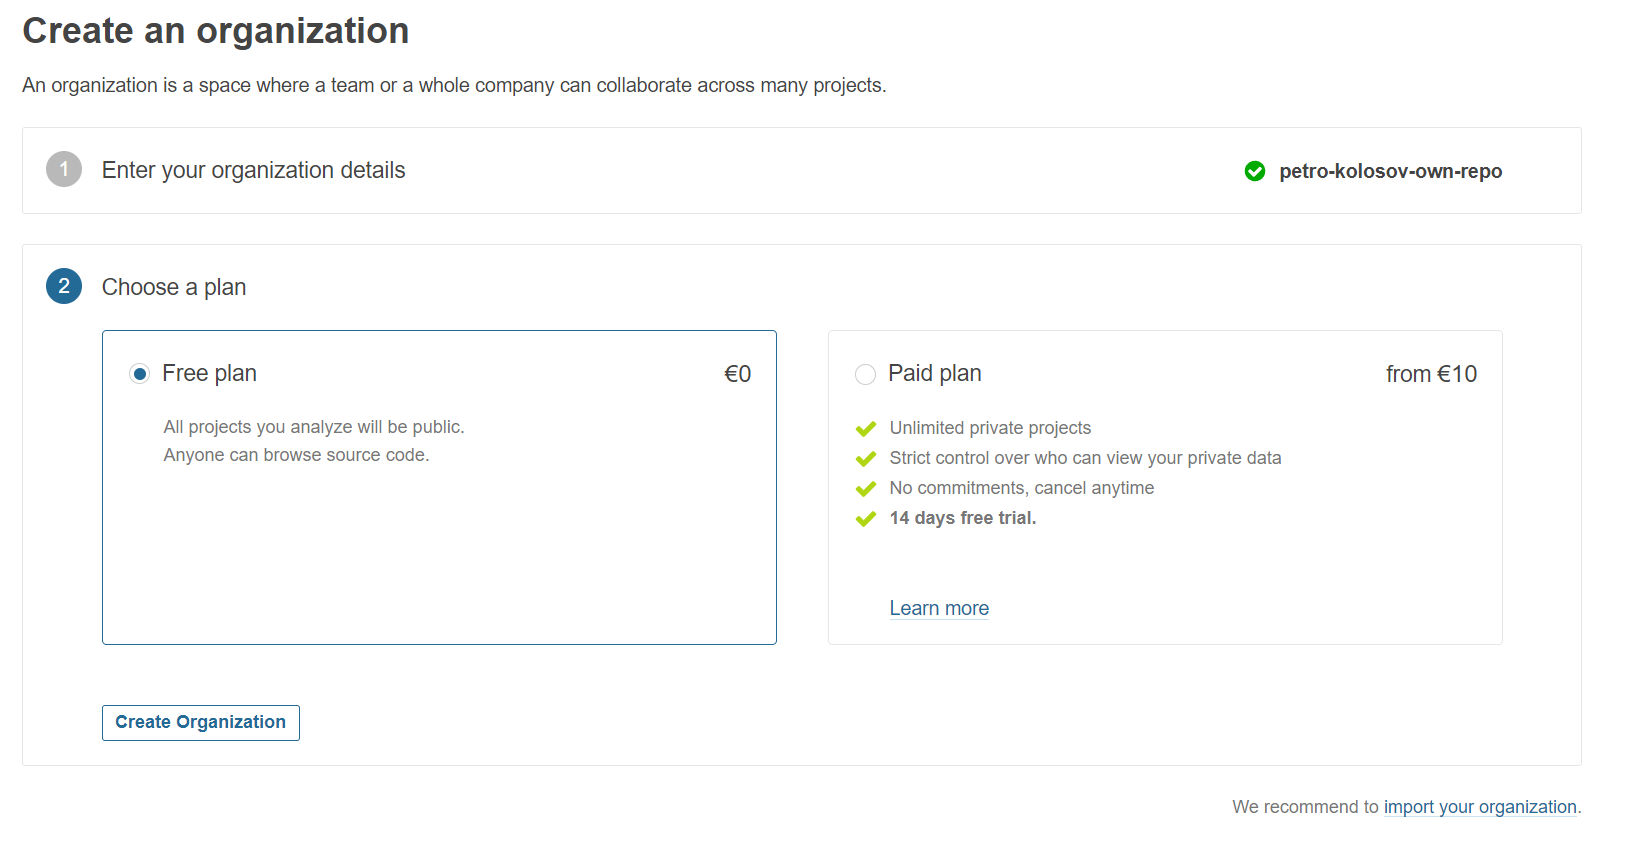
\includegraphics[width=1\textwidth]{img/04_choose_org_plan_free}
    ~\caption{Choose a plan for your organization.}\label{fig:figure4}
\end{figure}
Click create then, so we have finished second step, creating of the organization.

\subsection{Create a project on behalf of organization}\label{subsec:create-a-project-on-behalf-of-organization}
At your recently created organization, click the \texttt{Analyze new project} button
\begin{figure}[H]
    \centering
    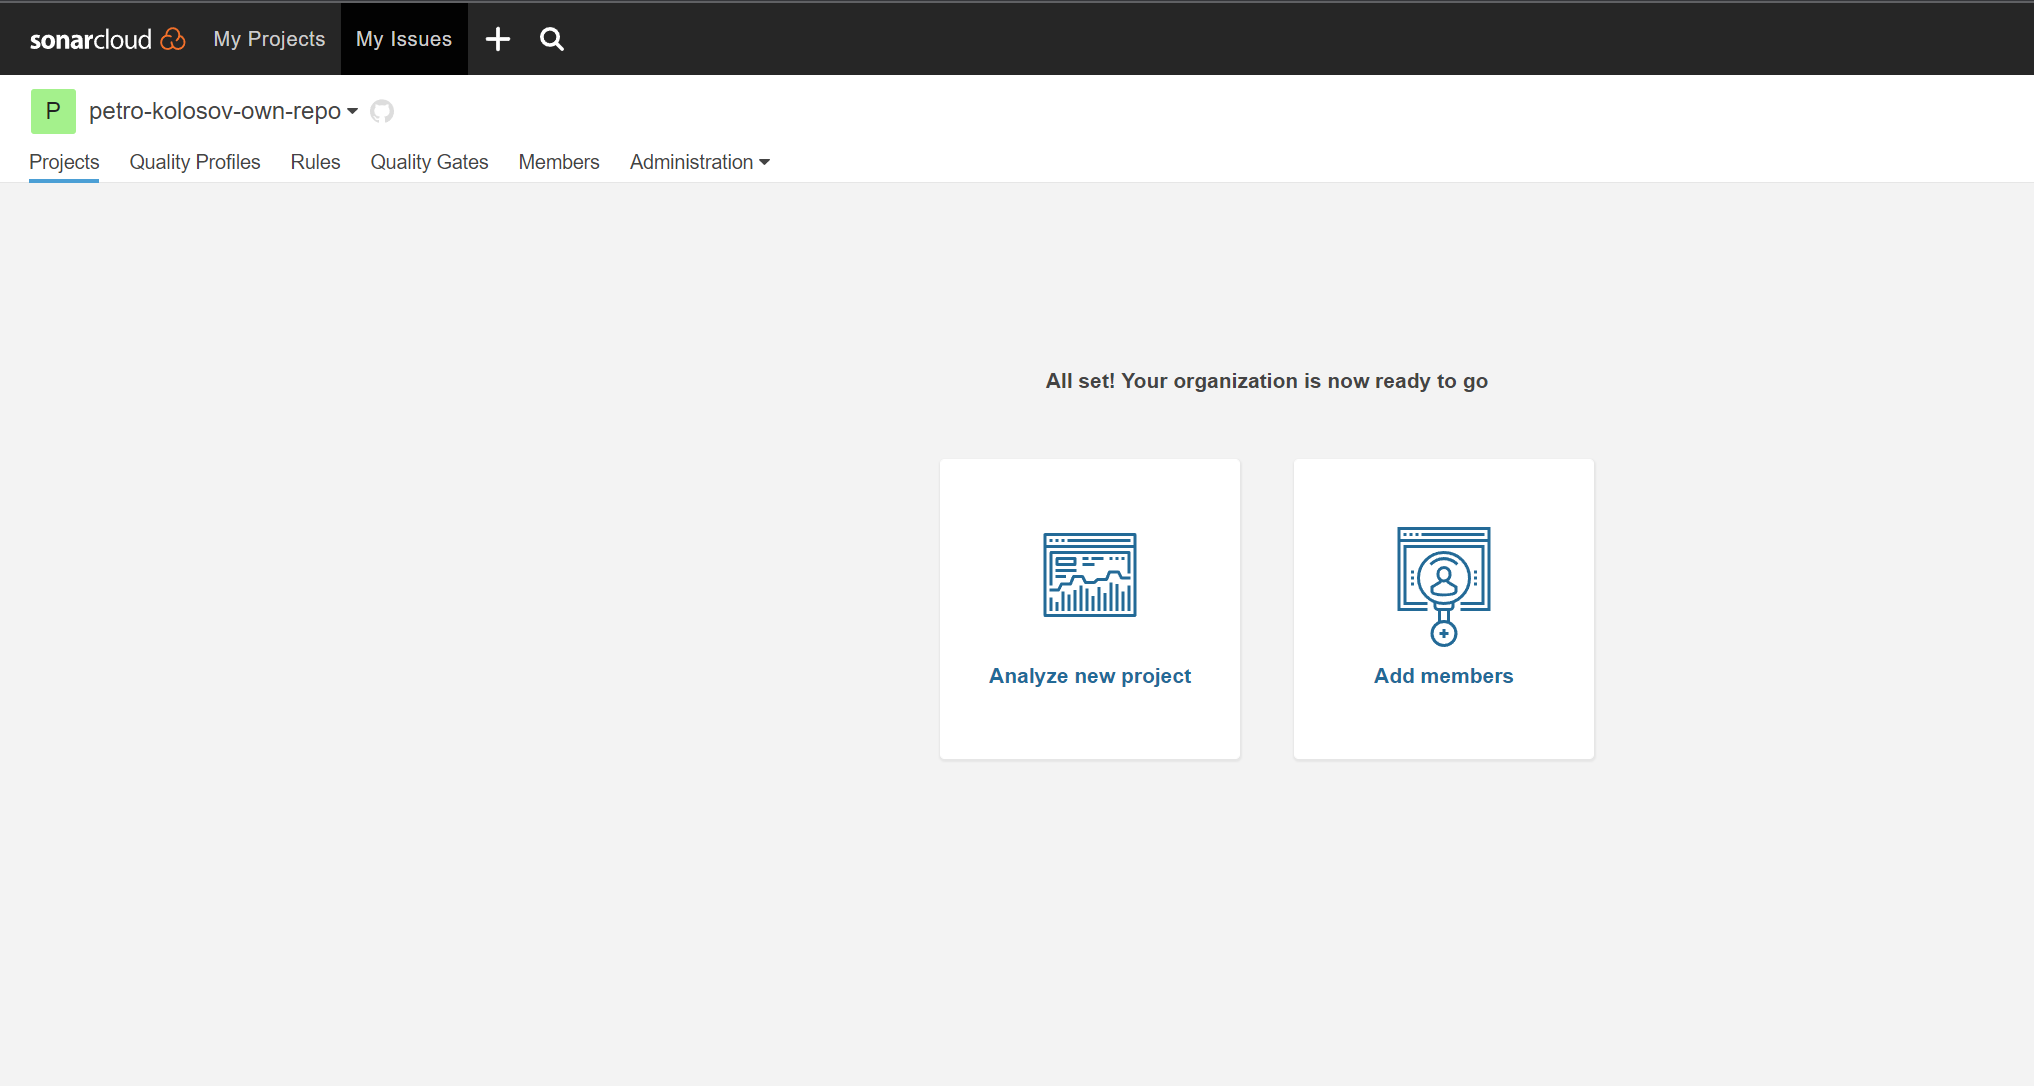
\includegraphics[width=1\textwidth]{img/05_organization_main_page}
    ~\caption{Click the \texttt{Analyze new project} button}\label{fig:figure5}
\end{figure}
Configure the name of your project
\begin{figure}[H]
    \centering
    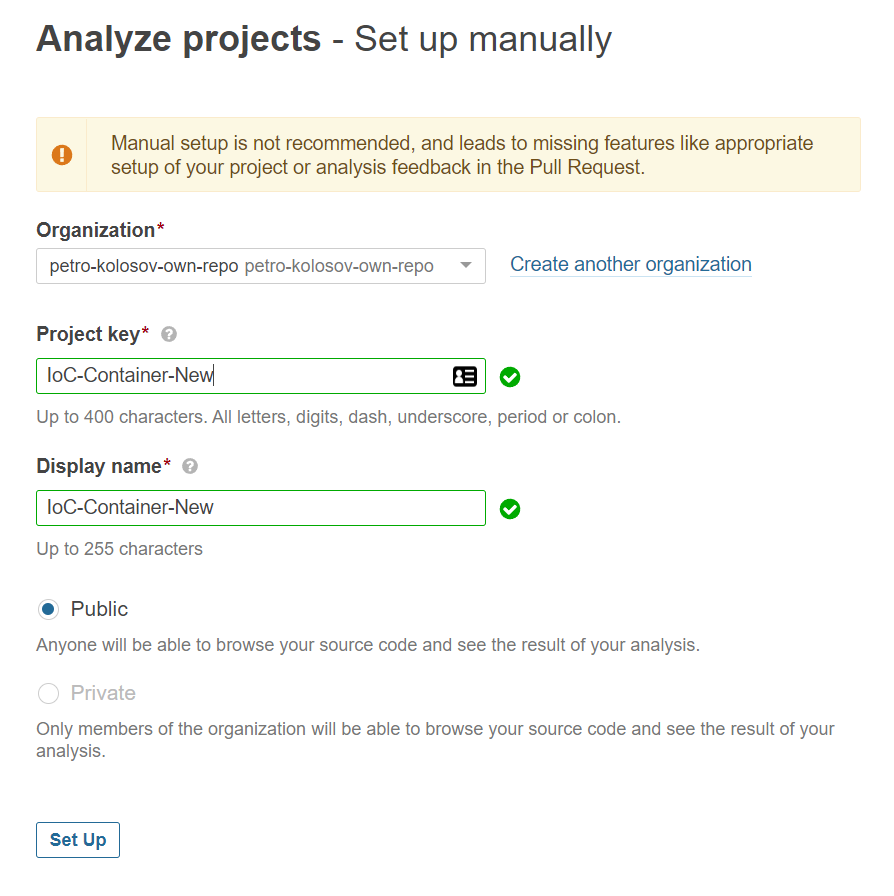
\includegraphics[width=0.5\textwidth]{img/06_configure_project_name}
    ~\caption{Configure the name of your project}\label{fig:figure6}
\end{figure}
Click \texttt{Set Up} and choose \texttt{Configure With Github Actions}, so that it looks like
\begin{figure}[H]
    \centering
    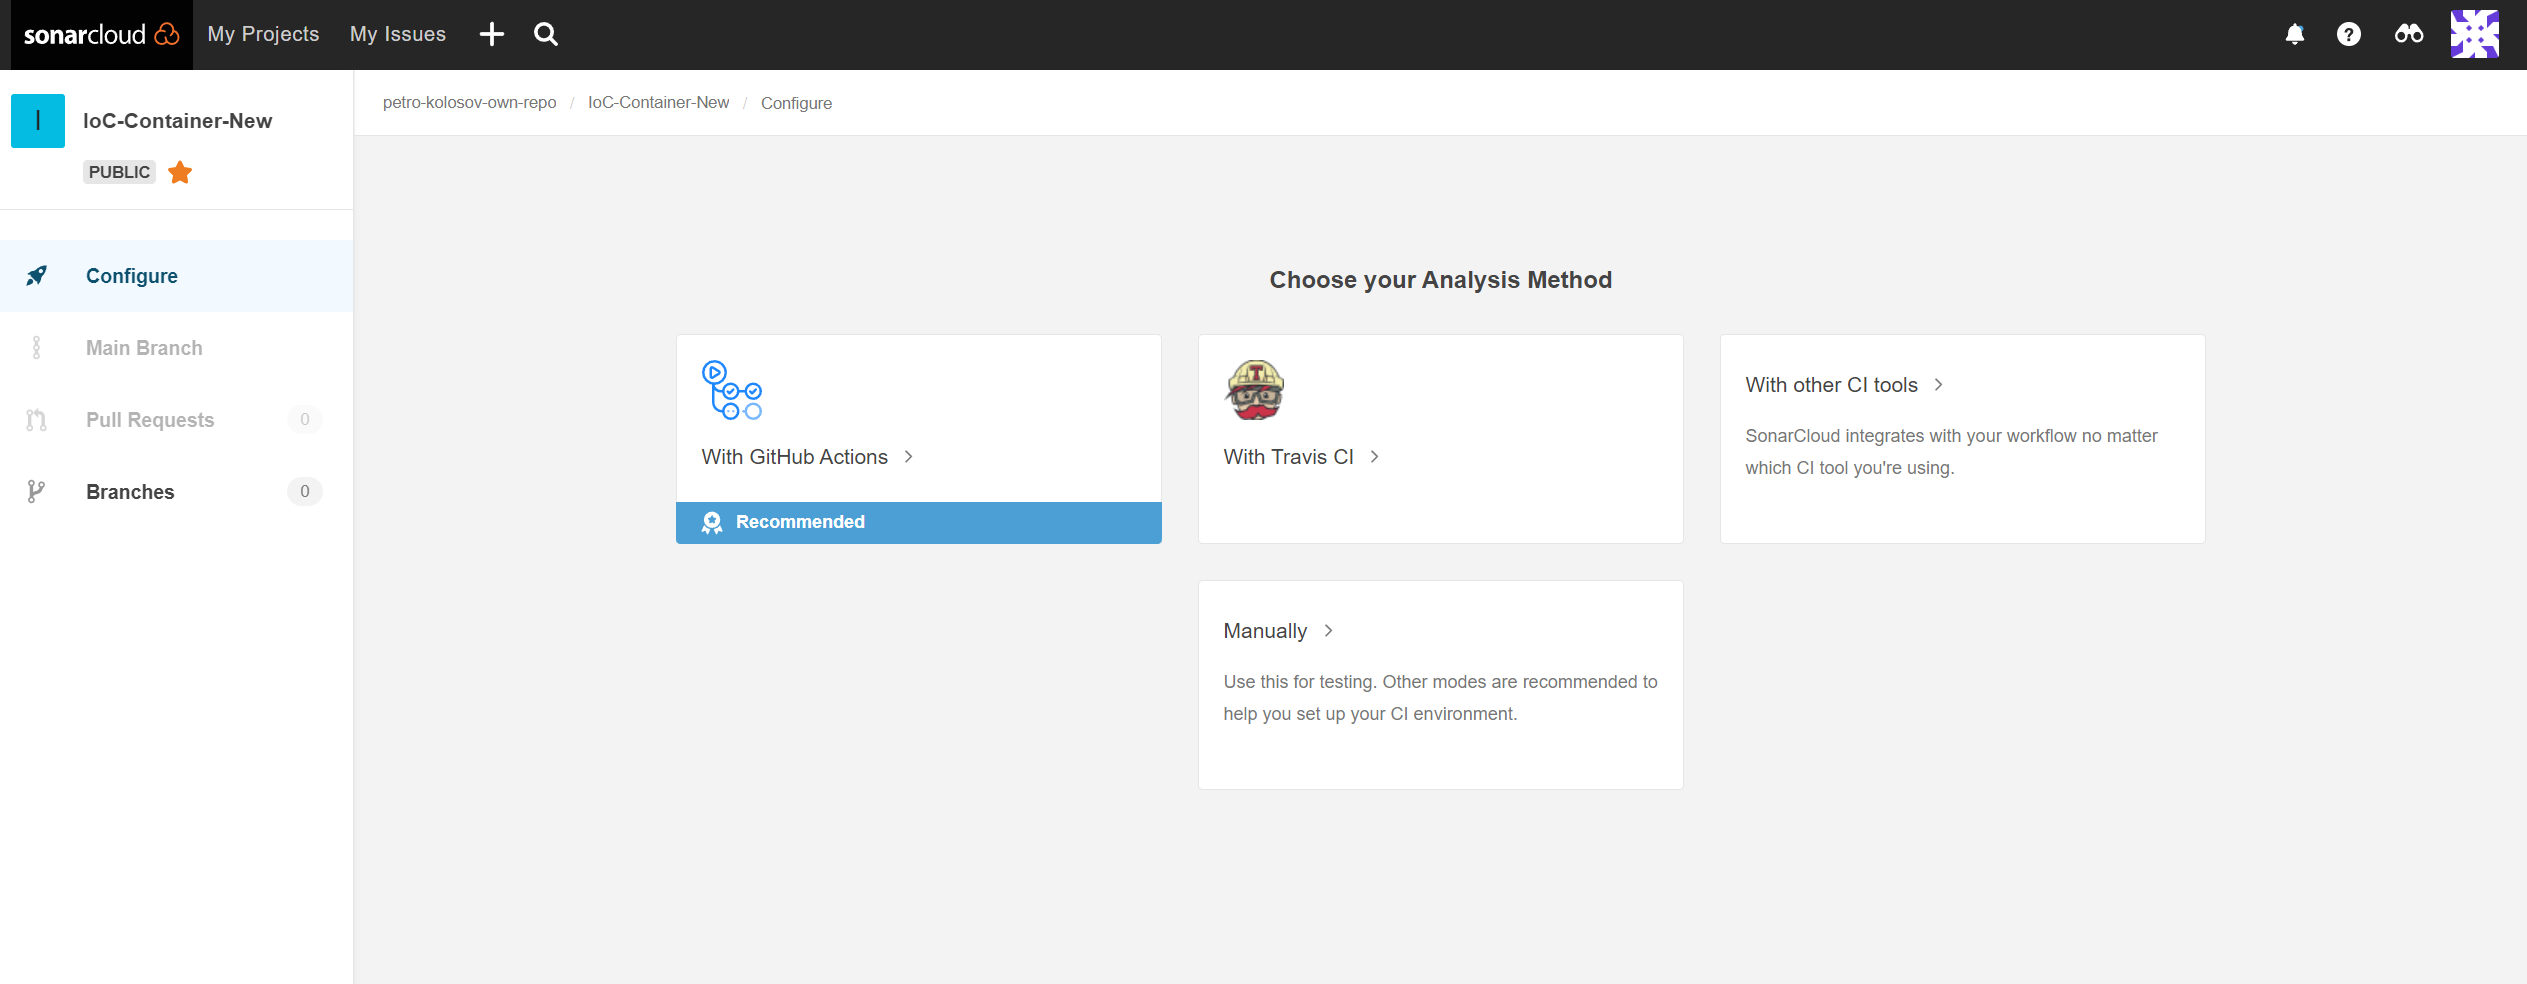
\includegraphics[width=1\textwidth]{img/07_configure_with_ghactions}
    ~\caption{\texttt{Configure With Github Actions}.}\label{fig:figure7}
\end{figure}
Create a specified GitHub actions secret at your repository on GitHub
\begin{figure}[H]
    \centering
    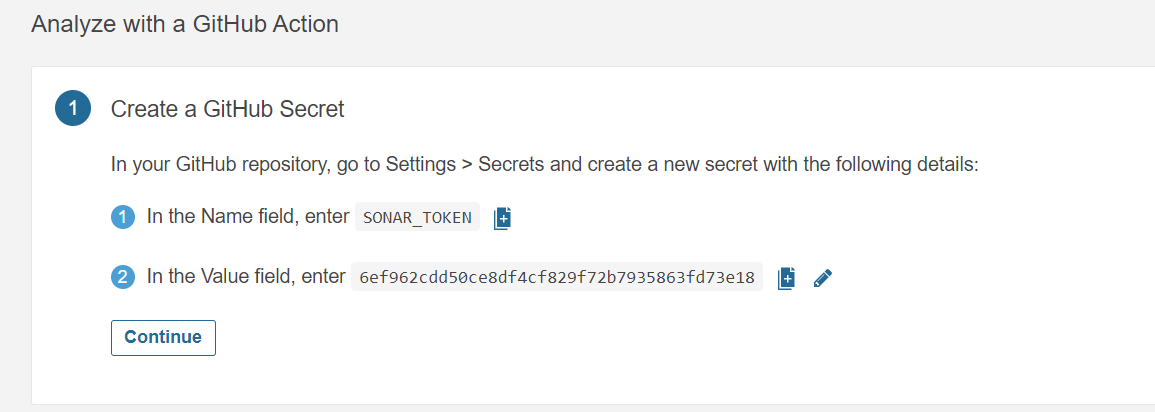
\includegraphics[width=1\textwidth]{img/08_set_github_actions_secret}
    ~\caption{Create a specified GitHub actions secret.}\label{fig:figure8}
\end{figure}
Do not worry, this key won't work and here just for example.
Clicking \texttt{Continue} and then \texttt{.NET} explores an example of the pipeline we are able to use
on the GitHub as an action of our repository.
\begin{figure}[H]
    \centering
    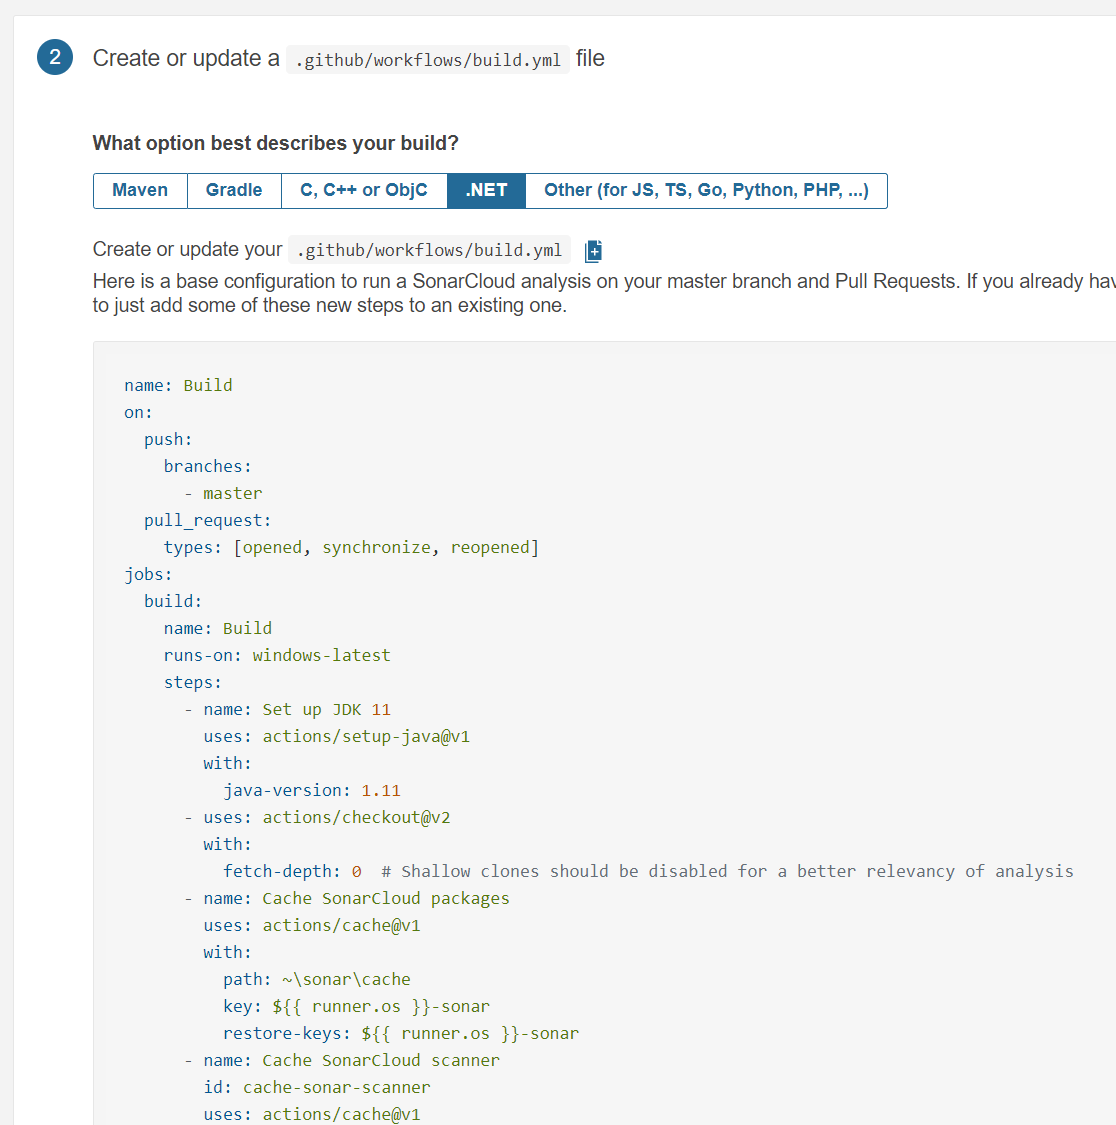
\includegraphics[width=1\textwidth]{img/09_pipeline_example}
    ~\caption{SonarCloud analyzer pipeline example.}\label{fig:figure9}
\end{figure}
Above pipeline runs on the \texttt{Windows} runner, but I prefer ubuntu runner for the reasons of performance
so that I change it following way
\begin{spverbatim}
name: Run SonarCloud analysis
on:
  push:
    branches: [ develop ]
  pull_request:
    types: [ opened, synchronize, reopened ]
  workflow_dispatch:
jobs:
  run-sonarcloud-analysis:
    name: Run SonarCloud Analysis
    runs-on: ubuntu-latest
    steps:
      - name: Set up JDK 11
        uses: actions/setup-java@v1
        with:
          java-version: 1.11
      - uses: actions/checkout@v2
        with:
          fetch-depth: 0

      - name: Cache SonarCloud packages
        uses: actions/cache@v1
        with:
          path: ~/sonar/cache
          key: ${{ runner.os }}-sonar
          restore-keys: ${{ runner.os }}-sonar

      - name: Cache SonarCloud scanner
        id: cache-sonar-scanner
        uses: actions/cache@v1
        with:
          path: ./.sonar/scanner
          key: ${{ runner.os }}-sonar-scanner
          restore-keys: ${{ runner.os }}-sonar-scanner

      - name: Setup .NET 6 SDK
        uses: actions/setup-dotnet@v1
        with:
          dotnet-version: 6.0.x

      - name: Install SonarCloud scanner
        if: steps.cache-sonar-scanner.outputs.cache-hit != 'true'
        run: |
          mkdir -p ./.sonar/scanner
          chmod a+rwx ./.sonar/scanner
          dotnet tool update dotnet-sonarscanner --tool-path ./.sonar/scanner

      - name: Analyze project
        run: |
          ./.sonar/scanner/dotnet-sonarscanner begin /k:"IoC-Container" /o:"petro-kolosov-own-repos" /d:sonar.login="${{ secrets.SONAR_TOKEN }}" /d:sonar.host.url="https://sonarcloud.io"
          dotnet build -c Release
          ./.sonar/scanner/dotnet-sonarscanner end /d:sonar.login="${{ secrets.SONAR_TOKEN }}"
        env:
          GITHUB_TOKEN: ${{ secrets.GITHUB_TOKEN }}
          SONAR_TOKEN: ${{ secrets.SONAR_TOKEN }}
\end{spverbatim}
After the push to the \texttt{develop} branch the action is triggered and succeeded
\begin{figure}[H]
    \centering
    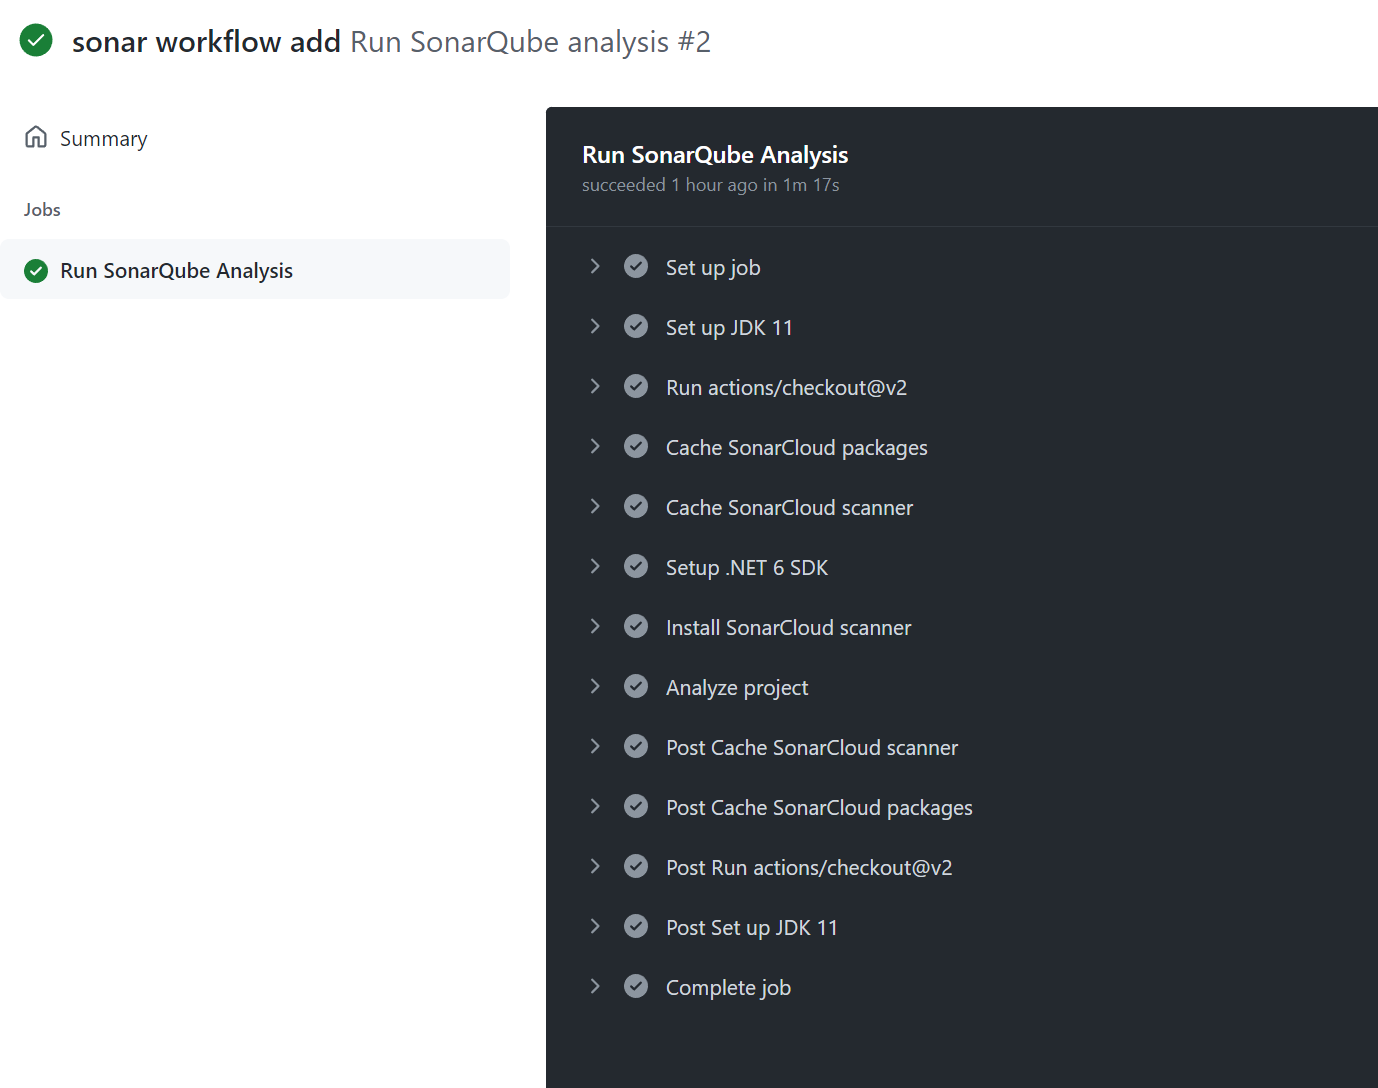
\includegraphics[width=0.6\textwidth]{img/10_action_screenshot}
    ~\caption{Action is triggered and succeeded.}\label{fig:figure10}
\end{figure}
So that pull request is analyzed and reported to the SonarCloud web application
\begin{figure}[H]
    \centering
    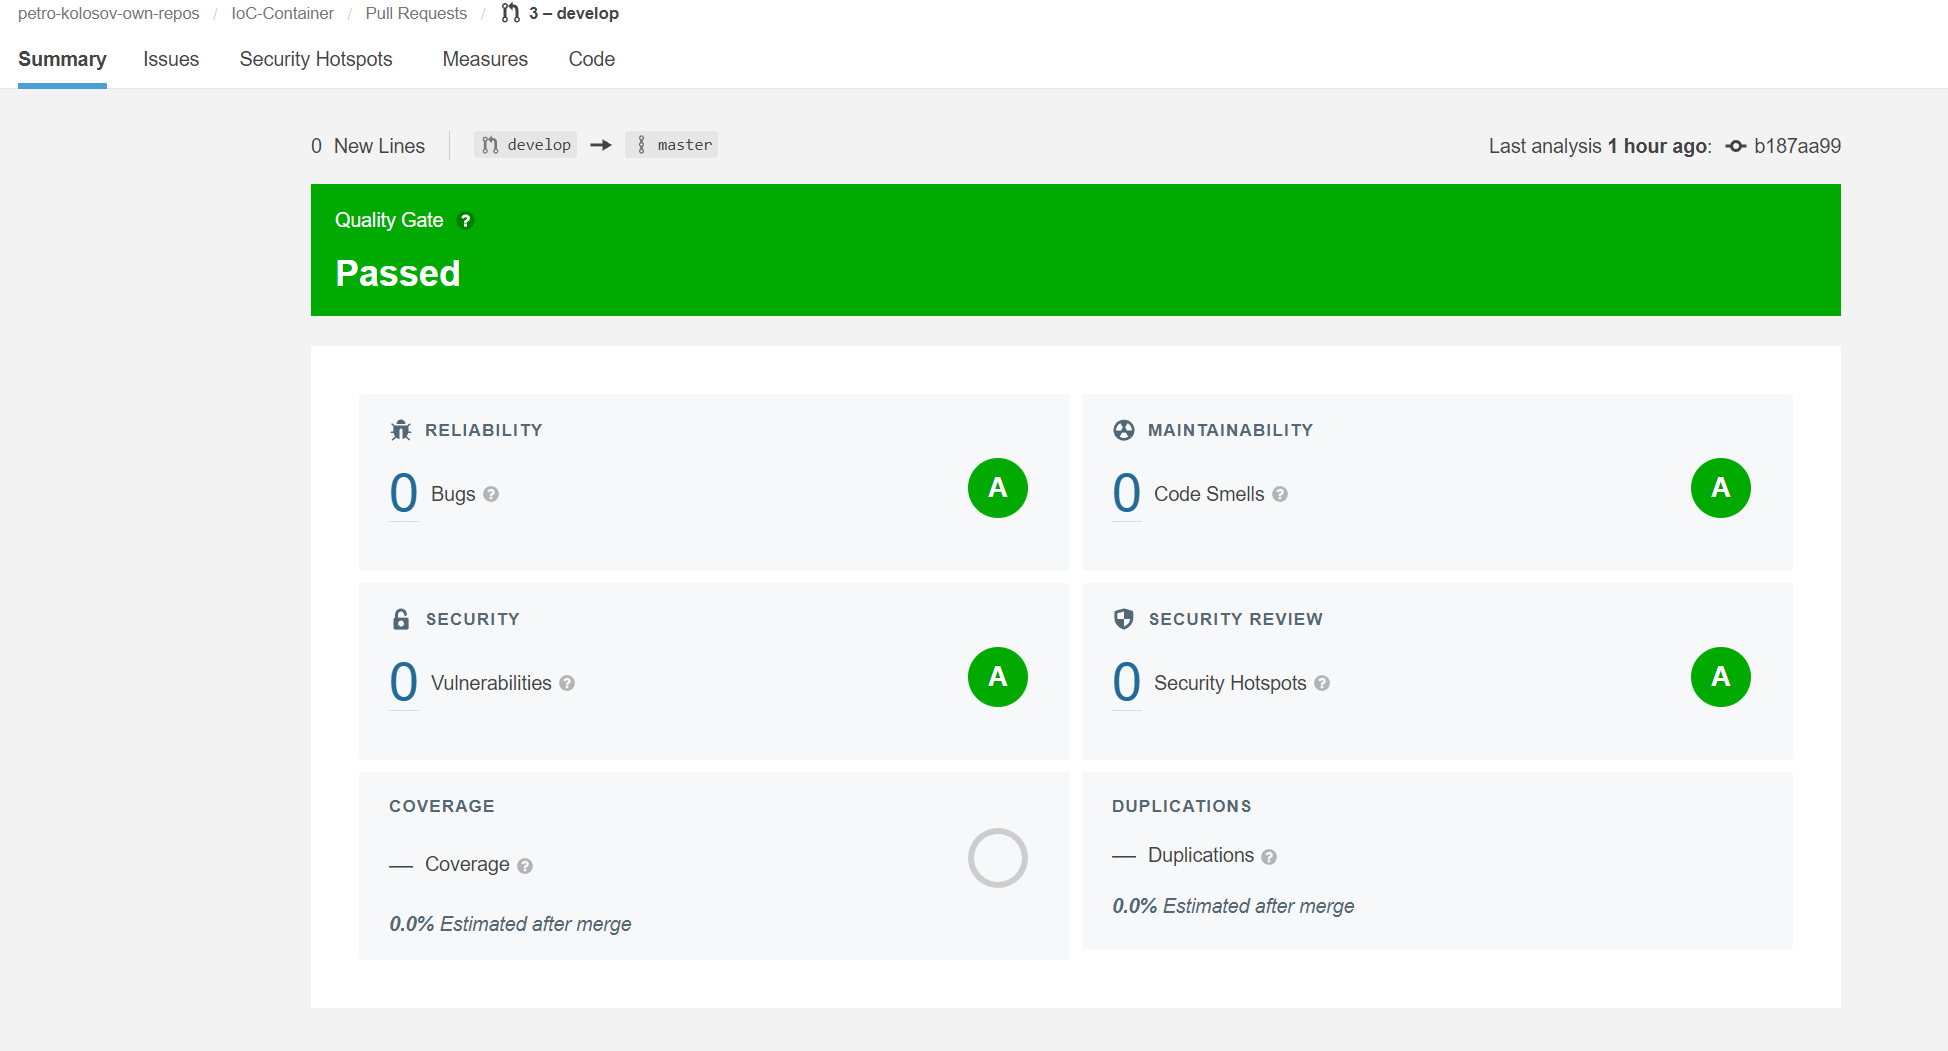
\includegraphics[width=1\textwidth]{img/11_pull_request_analyzed}
    ~\caption{Pull request analysis.}\label{fig:figure11}
\end{figure}
After merge workflow runs again in order to analyze the main branch \texttt{master} so that
we got a report as follows
\begin{figure}[H]
    \centering
    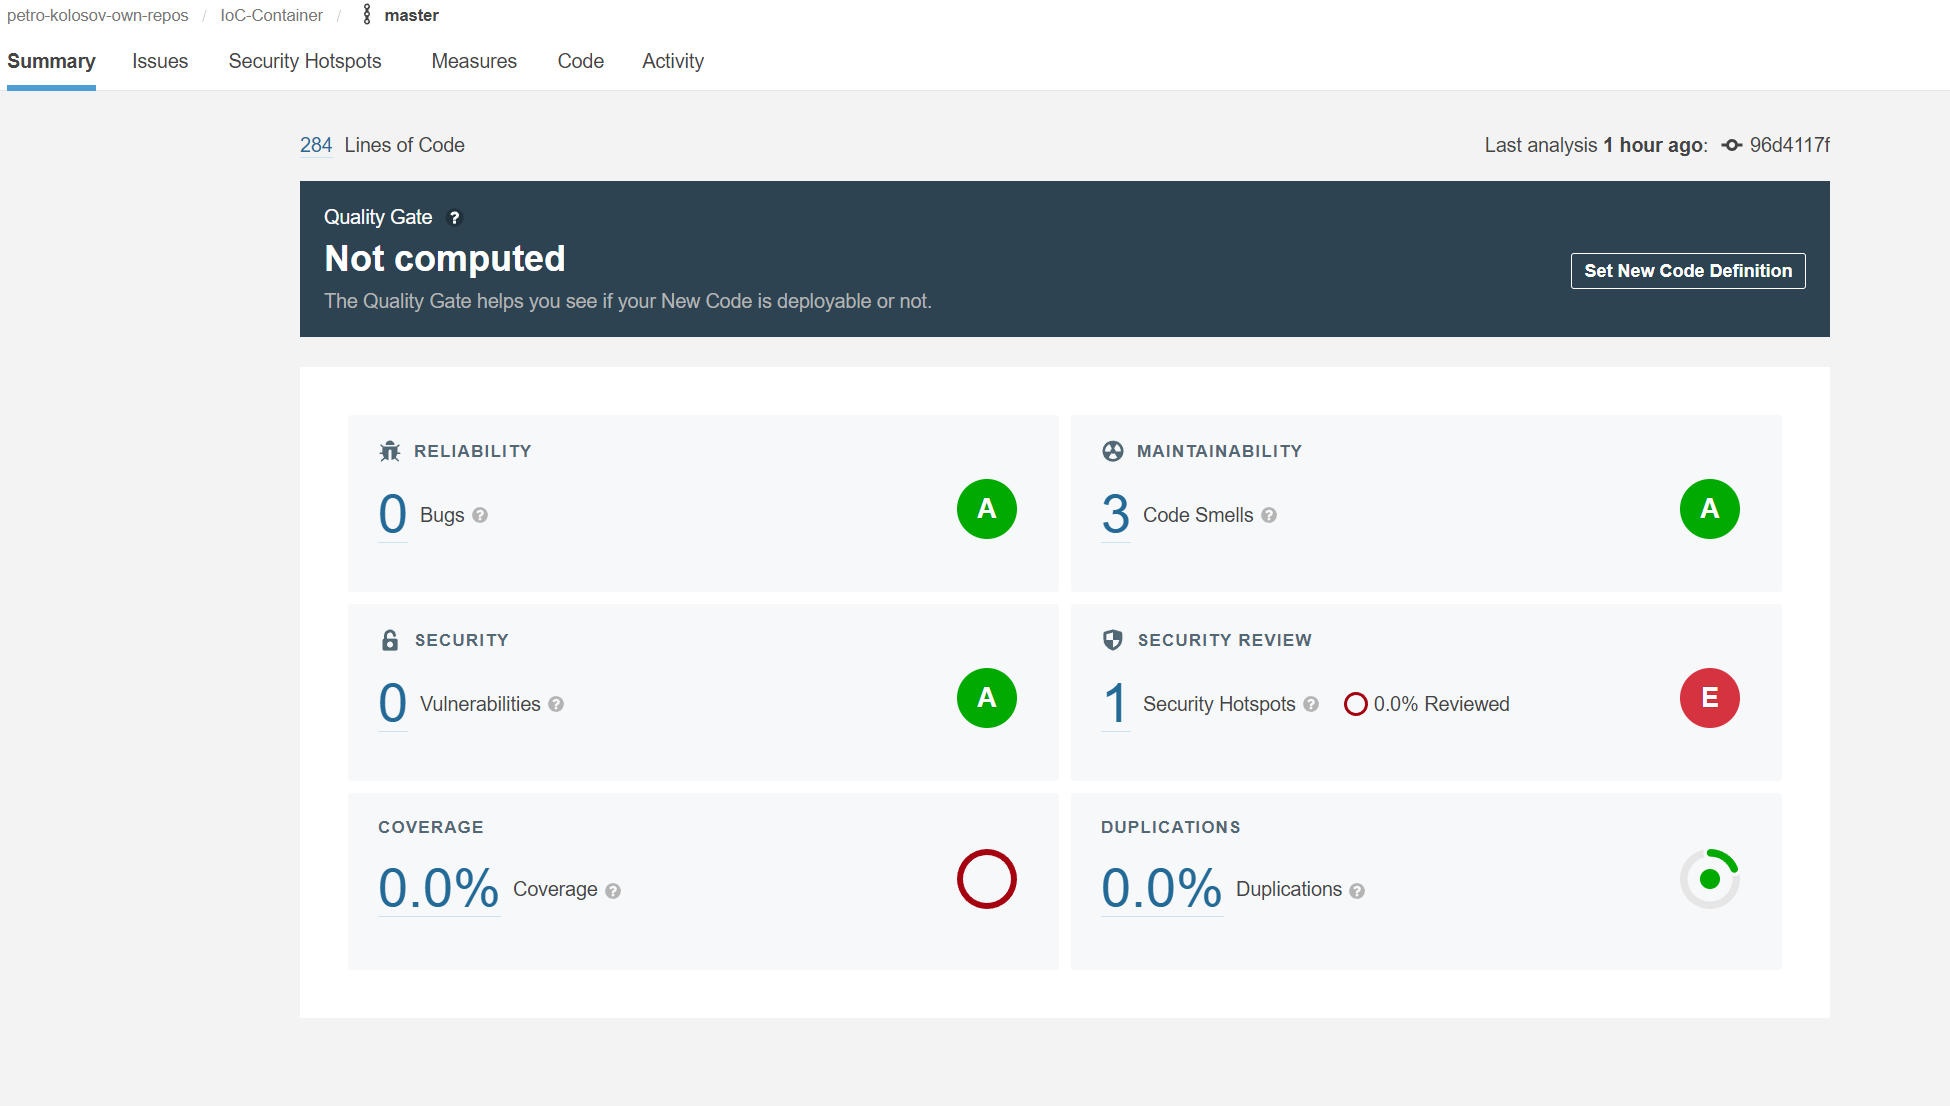
\includegraphics[width=1\textwidth]{img/12_main_branch_analyze}
    ~\caption{Main branch analysis.}\label{fig:figure12}
\end{figure}
Therefore, we have successfully established an integration between SonarCloud static code analyzer and GitHub repository.

\begin{itemize}
    \item \href{https://github.com/kolosovpetro/IoC-Container/blob/master/.github/workflows/run-sonarqube-analysis.yml}{\texttt{Workflow source}}
    \item \href{https://sonarcloud.io/project/overview?id=IoC-Container}{\texttt{SonarCloud dashboard}}
\end{itemize}